\documentclass[12pt,a4paper]{article}
\usepackage[utf8]{inputenc}
\usepackage[T2A]{fontenc}
\usepackage[russian]{babel}
\usepackage{amsmath,amssymb}
\usepackage{graphicx}
\usepackage{float}
\usepackage{caption}
\usepackage{booktabs}
\usepackage{array}
\usepackage{geometry}
\geometry{left=2cm,right=2cm,top=2cm,bottom=2cm}
\usepackage{siunitx}
\sisetup{output-decimal-marker={,}}
\usepackage{indentfirst}
\usepackage{setspace}
\onehalfspacing

\begin{document}

% Титульная страница
\begin{titlepage}
    \centering
    \vspace*{2cm}
    {\Large Московский физико-технический институт\\[0.5ex]
    (национальный исследовательский университет)\par}
    \vspace{1cm}
    {\large Кафедра общей физики\par}
    \vspace{2cm}
    {\LARGE \textbf{Лабораторная работа № 2.3.1}\par}
    \vspace{1cm}
    {\huge \textbf{Получение и измерение вакуума}\par}
    \vspace{3cm}
    \begin{flushright}
        \large
        Студент: \textit{Иванов Алексей}\\
        Группа: Б03-511\\
        Дата выполнения: 20.04.2026
    \end{flushright}
    \vfill
    Долгопрудный, 2026
\end{titlepage}

% Аннотация
\section*{Аннотация}
\textbf{Цель работы:} измерение объёмов форвакуумной и высоковакуумной частей установки; определение скорости откачки системы в стационарном режиме, а также по ухудшению и по улучшению вакуума.

\textbf{Оборудование:} вакуумная установка с форвакуумным и диффузионным насосами, масляный, термопарные и ионизационный манометры, капилляр, краны.


\section{Теоретические сведения}

\subsection{Критерии вакуума}
При нормальных условиях средняя длина свободного пробега молекул $\lambda \ll d$ (характерный размер установки). Критерий применимости сплошной среды — число Кнудсена:
\begin{equation}
    \mathrm{Kn} = \frac{\lambda}{d}.
\end{equation}
По значению $\mathrm{Kn}$ различают низкий ($\mathrm{Kn} \ll 1$), средний ($\mathrm{Kn} \sim 1$) и высокий ($\mathrm{Kn} \gg 1$) вакуум. По степени разрежения: низковакуумные установки — до $10^{-2}\text{--}10^{-3}$\ Торр, высоковакуумные — $10^{-4}\text{--}10^{-7}$\ Торр, сверхвысоковакуумные — $10^{-8}\text{--}10^{-11}$\ Торр.

\subsection{Экспериментальная установка}
Схема установки приведена на рис.~\ref{fig:scheme}. Основные элементы: форвакуумный баллон (ФБ), высоковакуумный диффузионный насос (ВН), высоковакуумный баллон (ВБ), масляный (М) и ионизационный (И) манометры, термопарные манометры (М1, М2), форвакуумный насос (ФН), краны К1--К6.

\begin{figure}[H]
    \centering
    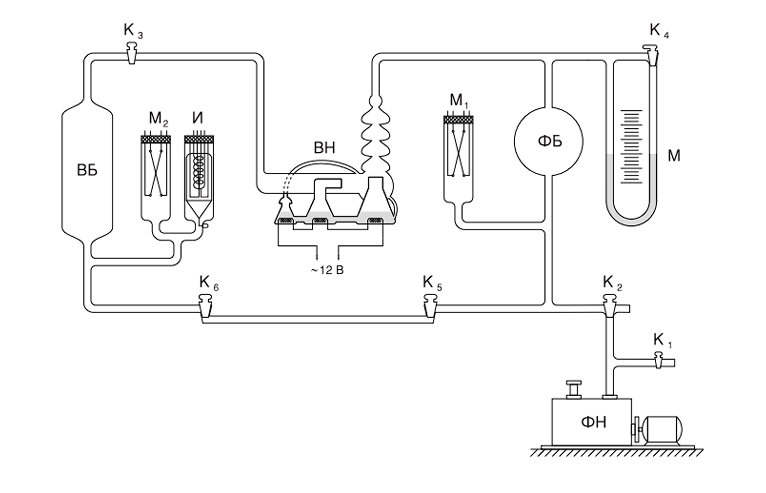
\includegraphics[width=0.8\textwidth]{уст.png}
    \caption{Схема экспериментальной установки.}
    \label{fig:scheme}
\end{figure}

Суммарный объём кранов К5 и К6 — 50\ см$^3$. Диаметр капилляра $d = 0,8$\ мм, длина $L = 108$\ мм.

\subsection{Процесс откачки}
Основное уравнение откачки:
\begin{equation}
    -V\,dP = (PW - Q_d - Q_n - Q_i)\,dt,
\end{equation}
где $Q_d$ — десорбция, $Q_n$ — натекание, $Q_i$ — обратный поток из насоса. При предельном вакууме $dP/dt = 0$:
\begin{equation}
    P_{\text{пр}} W = Q_d + Q_n + Q_i.
\end{equation}
Интегрирование при постоянных $W$ и потоках даёт:
\begin{equation}
    P - P_{\text{пр}} = (P_0 - P_{\text{пр}}) \exp\left(-\frac{W}{V}t\right).
\end{equation}
При $P_0 \gg P_{\text{пр}}$:
\begin{equation}
    P = P_0 \exp\left(-\frac{W}{V}t\right).
\end{equation}
Постоянная времени $\tau = V/W$.

При последовательном соединении элементов
\begin{equation}
    \frac{1}{W} = \frac{1}{W_{\text{н}}} + \frac{1}{C_1} + \frac{1}{C_2} + \dots
\end{equation}

\subsection{Течение разреженного газа через трубу}
В кнудсеновском режиме ($\lambda \gg d$) поток массы описывается формулой:
\begin{equation}
    \frac{d(PV)}{dt} = \frac{4}{3}r^3 \sqrt{\frac{2\pi RT}{\mu}} \frac{P_2 - P_1}{L}.
\end{equation}
Пренебрегая давлением на выходе, пропускная способность трубы:
\begin{equation}
    C_{\text{тр}} = \frac{4}{3} \frac{r^3}{L} \sqrt{\frac{2\pi RT}{\mu}}.
\end{equation}
Пропускная способность отверстия площадью $S$:
\begin{equation}
    C_{\text{отв}} = S \frac{\bar{v}}{4},
\end{equation}
где $\bar{v} = \sqrt{8kT/\pi m}$ — средняя тепловая скорость. Для воздуха при $T=293$\ К $\bar{v}/4 \approx 110$\ м/с $= 11$\ л/(с$\cdot$см$^2$).

Диффузионный насос работает аналогично кольцевому отверстию, откачивая со скоростью, определяемой площадью зазора между соплом и стенками.

\section{Обработка результатов измерений}

\subsection{Определение объёмов частей установки}
Атмосферное давление $P_{\text{а}} = 100,82$\ кПа. Плотность масла в манометре $\rho = 0,885$\ г/см$^3$.

Измерения для форвакуумной части:
\[
\Delta h_{\text{фв}} = h_1 - h_2 = (26,2 \pm 0,2)\ \text{см}.
\]
Давление в форвакуумной части после расширения:
\[
P_{\text{фв}} = \rho g \Delta h_{\text{фв}} = (2197,5 \pm 16,7)\ \text{Па}.
\]
По закону Бойля–Мариотта:
\[
V_{\text{фв}} = \frac{P_{\text{а}} V_{\text{заперт}}}{P_{\text{фв}}} = \frac{100,82 \cdot 10^3 \cdot 50 \cdot 10^{-6}}{2197,5} = (2,293 \pm 0,017)\ \text{л}.
\]

После открытия крана К3 и выравнивания давлений измерен полный объём:
\[
V_{\text{полн}} = (3,470 \pm 0,015)\ \text{л}.
\]
Тогда объём высоковакуумной части:
\[
V_{\text{вв}} = V_{\text{полн}} - V_{\text{фв}} = (1,180 \pm 0,022)\ \text{л}.
\]

\subsection{Предельный вакуум}
После откачки форвакуумным насосом до $\sim 2\cdot10^{-2}$\ Торр включён диффузионный насос. Ток подогрева: 0,6\ А (5 мин), затем 1,27\ А. Частота капель стекающего масла $\sim 12$\ мин$^{-1}$. После прогрева ионизационного манометра предельное давление:
\[
P_{\text{пр}} = 5,9 \cdot 10^{-5}\ \text{Торр}.
\]

\subsection{Скорость откачки по улучшению вакуума}
После закрытия крана К3 записывалось ухудшение вакуума до $\sim 6\cdot10^{-4}$\ Торр, затем кран открывался и фиксировалось улучшение. На рис.~\ref{fig:vacuum} представлены зависимости давления от времени в полулогарифмических координатах.

\begin{figure}[H]
    \centering
    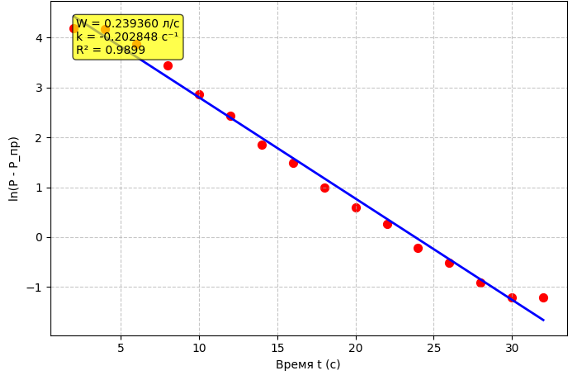
\includegraphics[width=0.8\textwidth]{улучшение.png}
    \caption{Улучшение вакуума.}
    \label{fig:vacuum}
\end{figure}

\begin{figure}[H]
    \centering
    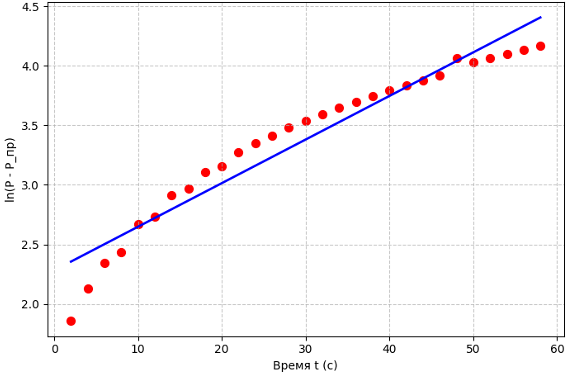
\includegraphics[width=0.8\textwidth]{ухудшение.png}
    \caption{Ухудшение вакуума.}
    \label{fig:vacuum}
\end{figure}

Линейная аппроксимация для процесса улучшения:
\[
\ln(P - P_{\text{пр}}) = 4,830 - 0,203 \cdot t.
\]
Согласно (4), наклон прямой равен $W/V_{\text{вв}}$, откуда:
\[
W = 0,203 \cdot 1,180 = (0,239 \pm 0,014)\ \text{л/с}.
\]

Для процесса ухудшения вакуума:
\[
\ln(P - P_{\text{пр}}) = 2,282 + 0,0366 \cdot t.
\]
Скорость натекания (по начальному линейному участку $P(t)$):
\[
\frac{dP}{dt} = 0,0366 \cdot (P - P_{\text{пр}}) \approx 6,8 \cdot 10^{-6}\ \text{Торр/с}.
\]
Поток натекания:
\[
Q_n + Q_d = \frac{dP}{dt} V_{\text{вв}} = (0,803 \pm 0,019) \cdot 10^{-5}\ \text{Торр}\cdot\text{л/с}.
\]

\subsection{Скорость откачки с помощью искусственной течи}
При открытии крана К6 установившееся давление:
\[
P_{\text{уст}} = 1,3 \cdot 10^{-4}\ \text{Торр}.
\]
Баланс потоков:
\[
(P_{\text{уст}} - P_{\text{пр}}) W = \frac{d(PV)_{\text{кап}}}{dt}.
\]
Поток через капилляр (формула (7)):
\[
\frac{d(PV)_{\text{кап}}}{dt} = \frac{4}{3} \left(\frac{d}{2}\right)^3 \sqrt{\frac{2\pi RT}{\mu}} \frac{P_{\text{ФВ}}}{L},
\]
где $P_{\text{ФВ}} \approx 10^{-2}$\ Торр. Подставляя числовые значения, получаем:
\[
W = 0,649\ \text{л/с}.
\]

\subsection{Сравнение результатов}
Значение $W = 0,239$\ л/с получено для системы «баллон + трубка + насос». При искусственной течи общая проводимость снижается из-за последовательного соединения капилляра и трубки. Различие в $\sim 2,7$ раза указывает на соизмеримость их пропускных способностей, что согласуется с оценкой $C_{\text{тр}} \sim 1$\ л/с по формуле (8).

\section{Выводы}
\begin{enumerate}
    \item Измерены объёмы форвакуумной ($2,29 \pm 0,02$\ л) и высоковакуумной ($1,18 \pm 0,02$\ л) частей установки.
    \item Достигнут предельный вакуум $P_{\text{пр}} = 5,9\cdot10^{-5}$\ Торр.
    \item По кривой улучшения вакуума определена скорость откачки $W = 0,239 \pm 0,014$\ л/с.
    \item Оценён поток натекания $Q_n \approx 0,8\cdot10^{-5}$\ Торр$\cdot$л/с.
    \item Методом искусственной течи получена оценка $W = 0,65$\ л/с; расхождение объяснено последовательным соединением газопроводящих элементов.
\end{enumerate}

\end{document}
